%!TEX root=..\main.tex
\newcolumntype{x}[1]{!{\centering\arraybackslash\vrule width #1}}


\pagebreak
\chapter{1. Übung Systhemsicherheit}
\section{Grundlagen des Debuggens}
Bis zur Eingabe ist die Zahl ''Input'' 0. In Zeile 8, also vor der Ausführung dieser Zeile, ist die Variable Input 23. Hier kann ein Breakpoint mit \texttt{b <Zeile>} gesetzt werden. Danach wird die ''super\_complicated\_function'' ausgeführt. Diese wird 4 mal aufgerufen und alle 2 ''Steps'' ändert sich Input. Den nächsten step erzwingt man mit dem Befehl \texttt{s} bzw. \texttt{step}. Den Wert der Variable erhält man mit \texttt{print input}. \\
23 $\rightarrow$ 230 $\rightarrow$ 644 $\rightarrow$ 1472 $\rightarrow$ 3144\\
3144 ist dann der letzte Wert, bis das Programm durchgelaufen ist.

\section{Manipulation des Programmzustandes}

In Zeile 8, wo beim nächsten ''Step'' die if-Abfrage ausgeführt wird, muss die Variable ''access\_level'' auf 1 verändert werden. Dies wird mit dem Befehl \texttt{set access\_level = 1} erreicht. Dieser Befehl verändert während der Ausführung des Programms die angegebene Variable. Die Flag aus der Funktion lautet \texttt{6952fb0c8b0ecf136b28705536794ced1c419599}

\section{Reverse Engineering 101}

\begin{figure}[h]
	\centering
	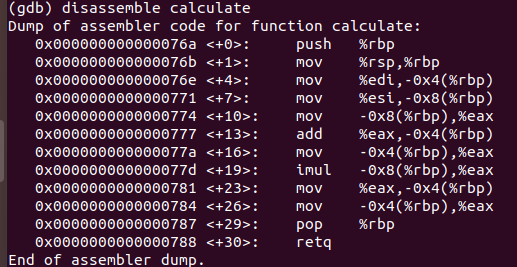
\includegraphics[width=0.6\textwidth]{figure/gdb}
\end{figure}

Dieser ''Assembler Dump'' kann erreicht werden, indem man folgende Befehle eingibt:
\begin{lstlisting}
gcc exercise03
gdb a.out
disessemble calculate
\end{lstlisting}

Der Befehl \textbf{gcc} ist ein Compiler, der eine C++ Datei nimmt und diese kompiliert. Nach dem Kompilieren wird der Debugger mittels \textbf{gdb} aufgerufen. Mit \textbf{disessemble} wird die angegebene Funktion auf Assembler-Level wiedergegeben.


